\chapter{Simultaneous imputation of missing data by multivariate predictive mean matching}
\chaptermark{Multivariate predictive mean matching}
\label{chap3}
	\begin{abstract}
		Predictive mean matching (PMM) is an easy-to-use and versatile univariate imputation approach. It is robust against transformations of the incomplete variable and violation of the normal model. However, univariate imputation methods cannot directly preserve multivariate relations in the imputed data. We wish to extend PMM to a multivariate method to produce imputations that are consistent with the knowledge of derived data (e.g., data transformations, interactions, sum restrictions, range restrictions, and polynomials). This paper proposes multivariate predictive mean matching (MPMM), which can impute incomplete variables simultaneously. Instead of the normal linear model, we apply canonical regression analysis to calculate the predicted value used for donor selection. To evaluate the performance of MPMM, we compared it with other imputation approaches under four scenarios: 1) multivariate normal distributed data, 2) linear regression with quadratic terms, 3) linear regression with interaction terms, 4) incomplete data with inequality restrictions. The simulation study shows that with moderate missingness patterns, MPMM provides plausible imputations and preserves relations in the data. This manuscript focuses on the all-or-none missing data pattern in the block. We also provide an algorithm for the more general case, and evaluating such an algorithm is subject to future work.   
	\end{abstract}

	\section{Introduction}
	\label{sec:3.1}
	Multiple imputation (MI) is a popular statistical method for the analysis of missing data problems. To provide valid inferences from the incomplete data, the analysis procedure of MI consists of three steps. First, in the imputation step, missing values are drawn from a plausible distribution (e.g., posterior distributions for Bayesian model-based approaches and a cluster of candidate donors for non-parametric and semi-parametric approaches) to generate several (\emph{m}) complete datasets. Historically the value of \emph{m} may have varied between 3 to 10 but now more are generally recommended, see \citet{white2011multiple} for a commonly cited rule of thumb (\emph{m} $\geq$ the percentage of incomplete cases). Second, in the analysis step, complete data analysis are used to estimate the quantity of scientific interest for each imputed data set. This step yields \emph{m} separate analyses because imputed datasets are different. Finally, in the pooling step, m results are aggregated into a single result by Rubin’s rules, accounting for the uncertainty of estimates due to the missing data \citep[p.76]{RubinD1987}. 
	
	Two widely used strategies for imputing multivariate missing data are joint modelling (JM) and fully conditional specification (FCS). Joint modelling was proposed by \citet{RubinD1987} and especially developed by \citet{schafer1997analysis}. Given that the data are assumed to follow a multivariate distribution, all incomplete variables are generally imputed by drawing from the joint posterior predictive distribution conditional on other variables. Fully conditional specification, which was developed by \citet{van1999multiple}, follows an iterative scheme that imputes each incomplete variable based on a conditionally specified model. Fully conditional specification allows for tremendous flexibility in multivariate model design and flexibility in imputing non-normal variables, especially discrete variables \citep{van2007multiple, goldstein2014fitting}. However, FCS may suffer from incompatibility problems, and computational shortcuts like the sweep operator cannot be applied to facilitate computation \citep{Buuren2018}. On the other hand, joint modelling possesses more solid theoretical guarantees. For a large number of incomplete variables, JM may lead to unrealistically large models and a lack of flexibility, which will not occur under FCS.  
	
	In practice, there are often extra structures in the missing data which are not modelled properly. Suppose there are two jointly missing variables $\boldsymbol{X_1}$ and $\boldsymbol{X_2}$. There may be restrictions on the sum of $\boldsymbol{X_1}$ and $\boldsymbol{X_1}$ (e.g., $\boldsymbol{X_1} + \boldsymbol{X_1} = C$, where $C$ is a fixed value) and the rank of $\boldsymbol{X_1}$ and $\boldsymbol{X_2}$ (e.g., $\boldsymbol{X_1} > \boldsymbol{X_2}$), data transformations (e.g., $\boldsymbol{X_2} = log(\boldsymbol{X_1})$, $\boldsymbol{X_2} = \boldsymbol{X_1}^2$) or interaction terms included in the data ($\boldsymbol{X_1}$, $\boldsymbol{X_2}$, $\boldsymbol{X_3}$ are jointly missing, where $\boldsymbol{X_3} = \boldsymbol{X_1} * \boldsymbol{X_2}$). In this paper, we focus on the missing data pattern where a set of variables are jointly observed or missing. This missing pattern is a simple scenario to illustrate.  
	
	The two popular approaches of MI mentioned before may not be appropriate for modelling the relations among multiple variables in the missing data. Joint modelling may lack the flexibility of modelling the relations explicitly, and FCS imputes each missing variable separately, which may not ensure that the imputation remains consistent with the observed relations among multiple variables. 
	
	\citet[section 4.7.2]{Buuren2018} suggested block imputation, which combines the strong points of joint modelling and fully conditional specification. The general idea is to place incomplete variables into blocks and apply multivariate imputation methods to the block. Joint modelling can be viewed as a ``single block" imputation method, where all variables are placed into the same block. In contrast, FCS is strictly a multiple blocks imputation method, where the number of blocks equals the number of incomplete columns in the data. It is feasible to consider the relations among a set of missing variables if we specify them as a single block and perform the MI iteratively over the blocks. 
	
	Based on the rationale of block imputation, we extend univariate predictive mean matching to the multivariate case to allow for the joint imputation of blocks of variables. The general idea is to match the incomplete case to one of the complete cases by applying canonical regression analysis and imputing the variables in a block entirely from the matched case \citep{little1988missing}. We shall refer to the multivariate extension of PMM as \emph{multivariate predictive mean matching} (MPMM).  
	
	Predictive mean matching (PMM) is a user-friendly and versatile semi-parametric imputation method. Multiple imputation by chained equation (\texttt{MICE}), which is a popular software package in \texttt{R} for imputing incomplete multivariate data by Fully Conditional Specification (FCS), sets the PMM as the default imputation approach for continuous variables \citep{Buuren2011}. We tailor PMM to the block imputation framework, which will widen its application. More computational details and properties of PMM would be addressed in section \ref{sec:3.2}.       
	
	
	For a comprehensive overview of missing data analysis, we refer to \citet{little2019statistical} for a comparison of approaches to missing data other than multiple imputation (e.g, ad-hoc methods, maximum likelihood estimation and weighting methods). \citet{schafer1999multiple}, \citet{sinharay2001use} and \citet{allison2001missing} introduced basic concepts and general methods of MI. \citet{schafer2002missing} discussed practical issues of application of MI. Various sophisticated missing data analysis were developed on the fields of multilevel model \citep{longford2001multilevel}, structural equation modelling \citep{olinsky2003comparative, allison2003missing}, longitudinal data analysis \citep{twisk2002attrition, demirtas2004modeling} and meta-analysis \citep{pigott2001missing}. \citet{schafer2003multiple} compared Bayesian MI methods with maximum likelihood estimation. \citet{seaman2013review} gave an overview of the use of inverse probability weighting in missing data problems. \citet{ibrahim2005missing} provided a review of various advanced missing data methods. MI as well as other approaches are now being applied in many fields (e.g., epidemiology, psychology, and sociology) and implemented in many statistical software packages (e.g., \texttt{mice} and \texttt{mi} in \texttt{R}, \texttt{IVEWARE} in \texttt{SAS}, \texttt{ice} in \texttt{STATA} and module \texttt{MVA} in \texttt{SPSS}) \citep{Buuren2011}.
	
	
	
	The following section will outline canonical regression analysis, introduce predictive mean matching (PMM), and connect the techniques to propose multivariate predictive mean matching (MPMM). Section \ref{sec:3.3} provides a simple comparison between PMM and MPMM. Section \ref{sec:3.4} is a simulation study investigating whether MPMM yields valid estimates and preserves functional relations between imputed values. The discussion closes the paper.
	
	
	
	
	
	\section{Multivariate Predictive Mean Matching}
	\label{sec:3.2}
	\subsection{Canonical regression analysis (CRA)}
	Canonical regression analysis is a derivation and asymmetric version of canonical correlation analysis (CCA). It aims to look for a linear combination of covariates that predicts a linear combination of outcomes optimally in a least-squares sense \citep{Israels1987}. The basic idea of canonical regression analysis is quite old and has been discussed under different names, such as Rank-reduced regression \citep{izenman1975reduced} and partial least squares \citep{sun2009equivalence}.  
	
	Let us consider the equation
	\begin{equation}
		\boldsymbol{\alpha'Y} = \boldsymbol{\beta X} + \epsilon.
	\end{equation}
	We aim to minimize the variance $\epsilon$ with respect to $\alpha$ and $\beta$ under some restrictions. CRA can be implemented by maximizing the squared multiple correlation coefficient for the regression of $\alpha'Y$ on $X$, which can be written as
	\begin{equation}
		R^2_{\alpha'y.x}=\frac{\boldsymbol{\alpha'\Sigma_{yx}\Sigma^{-1}_{xx}\Sigma_{xy}\alpha}}{\boldsymbol{\alpha'\Sigma_{yy}\alpha}},
	\end{equation}
	where $R^2_{\alpha'y.x}$ is the ratio of the amount of variance of $\boldsymbol{\alpha'Y}$ accounted for by the covariates $\boldsymbol{X}$ to the total variance. According to \citet{McDonald1968}, maximization of the above equation leads to eigenvalue decomposition. The solution is that $\boldsymbol{\alpha}$ is the right-hand eigenvector of $\boldsymbol{\Sigma^{-1}_{yy}\Sigma_{yx}\Sigma^{-1}_{xx}\Sigma_{xy}}$ corresponding to its greatest eigenvalue. After reducing the rank of $\boldsymbol{\alpha'Y}$ to $1$, we could estimate $\boldsymbol{\beta}$ by multivariate regression analysis. 
	
	\subsection{Predictive mean matching (PMM)}
	PMM was first proposed by \citet{rubin1986statistical} and formalized by \citet{little1988missing}. It can be viewed as an extension of the $k$ nearest neighbour method. PMM calculates the estimated value of the missing variable through a specified imputation model (e.g., linear imputation model). The method selects a set of candidate donors (typically, the number of candidate donors is 5) from all complete cases whose estimated values are closest to the estimated value of the missing unit. The unobserved value is imputed by randomly drawing one of the observed values of the candidate donors \citep{Buuren2018}.
	
	\subsubsection{Computational details}
	We elaborate the algorithm of univariate predictive mean matching for the clear illustration of its merger with canonical regression analysis \citep{Vink2015}. $\boldsymbol{X_{obs}}$, a $N_{obs} \times j$ matrix, denotes the observed part of predictors and $\boldsymbol{X_{mis}}$, a $N_{mis} \times j$ matrix, denotes the missing part of predictors. 
	\begin{enumerate}
		\item Use linear regression of $\boldsymbol{Y_{obs}}$ given $\boldsymbol{X_{obs}}$ to estimate $\boldsymbol{\hat{\beta}}$ and $\hat{\epsilon}$ through ordinary least squares
		\item Draw $\sigma^{2\ast}=\hat{\epsilon}^\mathsf{T}\hat{\epsilon}/A$, where $A$ is a $\chi^2$ variate with $N_{obs}-j$ degrees of freedom
		\item Draw $\boldsymbol{\beta^{\ast}}$ from a multivariate normal distribution with mean vector $\boldsymbol{\hat{\beta}}$ and covariance matrix $\boldsymbol{\sigma^{2\ast}(X^\mathsf{T}_{obs}X_{obs})^{-1}}$
		\item Calculate $\boldsymbol{\hat{V}_{obs}=X_{obs}\hat{\beta}}$ and $\boldsymbol{\hat{V}_{mis}=X_{mis}\beta^{\ast}}$
		\item For each missing cell $y_{mis,n}$, where $n=1,\cdots,N_{mis}$
		\begin{enumerate}
			\item Find $\Delta=|\hat{v}_{mis,n}-\hat{v}_{obs,k}|$ for all $k=1,\cdots,N_{obs}$
			\item Pick several observed entries $y_{obs}$, 5 as default in \emph{mice.impute.pmm}, with the smallest distance defined in step 5(a)
			\item Randomly draw one of the $y_{obs}$ which are picked in the previous step to impute $y_{mis,n}$  
		\end{enumerate}
		\item Repeat steps 1-5 \emph{m} times and save \emph{m} completed datasets. 
	\end{enumerate}
	
	Predictive mean matching has been proven to perform well in a wide range of simulation studies and is an attractive way to impute missing data \citep{Buuren2011, Vink2015, Heitjan1991, Morris2014, Vink2014}. More precisely, PMM has the appealing feature that the imputed values are always within the range of observed data because imputed values are replaced by real observed values \citep{Buuren2018}. For the same reason, PMM yields acceptable imputations even when normality assumptions are violated \citep{Vink2014}. PMM is good at preserving the distributional shape. If observations are strictly positive, so will the imputations from PMM be. Furthermore, since PMM is a semi-parametric technique, it alleviates the adverse impact when the imputation model is misspecified \citep{JamesR.Carpenter2013}. 
	
	Although PMM was developed for situations with only a single incomplete variable, it is easy to implement it under a fully conditionally specification framework for imputing multivariate missing data. However, the application of PMM under the FCS framework is only limited to univariate imputation. Therefore, it may distort the multivariate relations in the imputations and narrow the application of the method to more complex data structures. For example, \citet{seaman2012multiple} concluded that a univariate implementation of predictive mean matching is not advised to produce plausible estimates when the analysis model contains non-linear terms. As a multivariate extension to PMM, we expect that MPMM could yield plausible and consistent imputations when the missing covariates include polynomial or interaction terms.  
	
		
	\subsection{Multivariate predictive mean matching (MPMM)}
	\label{sec:3.2.3}
	For illustration, we present the algorithm with one missing data pattern. The appendix discusses the extension to cases with multiple missing patterns. 
	Let $\boldsymbol{Y=(Y_1,\cdots,Y_I)}$ and $\boldsymbol{X=(X_1,\cdots,X_J)}$ be two sets of $I$ jointly incomplete variables and $J$ complete  quantitative variables, respectively. Let $\boldsymbol{V = \alpha Y}$ denotes the linear combination of multiple response variables and $\boldsymbol{X}$ denotes predictors with $j$ dimensions. 
	\begin{enumerate}
		\item Use the observed data to estimate the $(I+J)\times(I+J)$ covariance matrix
		\[ \left( \begin{array}{cc}
			\boldsymbol{\Sigma_{y_{obs}y_{obs}}} & \boldsymbol{\Sigma_{y_{obs}x_{obs}}}  \\
			\boldsymbol{\Sigma_{x_{obs}y_{obs}}} & \boldsymbol{\Sigma_{x_{obs}x_{obs}}}  \end{array} \right)\]
		\item Find the largest eigenvalue $\lambda^2$ of $\boldsymbol{\Sigma^{-1}_{y_{obs}y_{obs}}\Sigma_{y_{obs}x_{obs}}\Sigma^{-1}_{x_{obs}x_{obs}}\Sigma_{x_{obs}y_{obs}}}$ and its corresponding right-hand eigenvector $\alpha$
		\item Calculate the linear combination $\boldsymbol{\alpha'Y}$ for all completely observed individuals in the sample: $\boldsymbol{V_{obs}=\alpha'Y_{obs}}$ 
		\item Use linear regression of $\boldsymbol{V_{obs}}$ given $\boldsymbol{X_{obs}}$ to estimate $\boldsymbol{\hat{\beta}}$ and $\hat{\epsilon}$ through ordinary least squares
		\item Draw $\sigma^{2\ast}=\hat{\epsilon}^\mathsf{T}\hat{\epsilon}/A$, where $A$ is a $\chi^2$ variate with $N_{obs}-j$ degrees of freedom
		\item Draw $\beta^{\ast}$ from a multivariate normal distribution with mean vector $\boldsymbol{\hat{\beta}}$and covariance matrix $\boldsymbol{\sigma^{2\ast}(X^\mathsf{T}_{obs}X_{obs})^{-1}}$
		\item Calculate $\boldsymbol{\hat{V}_{obs}=X_{obs}\hat{\beta}}$ and $\boldsymbol{\hat{V}_{mis}=X_{mis}\beta^{\ast}}$
		\item For each missing vector $\boldsymbol{y_{mis,n}}$, where $n=1,\cdots,N_{mis}$
		\begin{enumerate}
			\item Find $\Delta=|\hat{v}_{mis,n}-\hat{v}_{obs,k}|$ for all $k=1,\cdots,N_{obs}$
			\item Pick several observed components $y_{obs} = \{y_{1, obs},\cdots,y_{I, obs}\}$, 5 as default, with the smallest distance defined in step 8(a)
			\item Randomly draw one of the $y_{obs}$ which are picked in the previous step to impute $y_{mis,n}$ 
		\end{enumerate}
		\item Repeat steps 5-8 \emph{m} times and save \emph{m} completed datasets.
	\end{enumerate}
	
	We also tried other methods of multivariate analysis, such as multivariate regression analysis (MRA) \citep[chapter 10]{rencher2003methods} and redundancy analysis (RA) \citep{van1977redundancy}. However, imputation models specified by MRA or RA are not appropriate because of the assumed independence between missing variables. The violation of this assumption leads to less sensible imputations when there are extra relations among missing covariates. 
	
	\section{Comparison between PMM and MPMM}
	\label{sec:3.3}
	We shall illustrate that although MPMM is a multivariate imputation method, where the whole missing component is assigned entirely from the matching donor, the derived imputed datasets are also plausible when targets of interest only involve a subset of variables ($E(\boldsymbol{Y_{1}})$, $\rho(\boldsymbol{Y_{1}}, \boldsymbol{Y_{2}})$) in the block. 
	
	\subsection{Simulation conditions}
	The predictors were generated by a multivariate distribution  
	\begin{eqnarray*}
		\begin{pmatrix}\boldsymbol{X_{1}}\\
			\boldsymbol{X_{2}}\\
			\boldsymbol{X_{3}}
		\end{pmatrix} & \sim & \mathcal{N}\left[\left(\begin{array}{c}
			2\\
			2\\
			2
		\end{array}\right),\left(\begin{array}{ccc}
			12 & 0 & 0\\
			0 & 12 & 0\\
			0 & 0 & 12
		\end{array}\right)\right].\\
	\end{eqnarray*}
	The responses were generated based on the multivariate linear model
	\begin{eqnarray*}
		\begin{pmatrix}\boldsymbol{Y_{1}}\\
			\boldsymbol{Y_{2}}\\
			\boldsymbol{Y_{3}}
		\end{pmatrix} & \sim & \mathcal{N}\left[\left(\begin{array}{c}
			3\boldsymbol{X_1} + \boldsymbol{X_2} + 2\boldsymbol{X_{3}}\\
			\boldsymbol{X_{1}} + 5\boldsymbol{X_{2}} + 2\boldsymbol{X_{3}}\\
			5\boldsymbol{X_{1}} + 3\boldsymbol{X_{2}} + \boldsymbol{X_{3}}
		\end{array}\right),\left(\begin{array}{ccc}
			4 & 4\rho & 4\rho\\
			4\rho & 4 & 4\rho\\
			4\rho & 4\rho & 4
		\end{array}\right)\right],\\
	\end{eqnarray*}
	where $\rho$ denotes the correlation between the predictors $\boldsymbol{X}$. Let \textbf{R} be the vector of observation indicators whose values are zero if the corresponding variable is missing and one if observed. We simulated missingness such that rows in the set $(\boldsymbol{Y_1, Y_2, Y_3})$ were always either observed or completely missing. This joint missingness was either completely at random (MCAR) with $P(\textbf{R}=0|\textbf{X}, \textbf{Y})=0.4$ or right-tailed missing at random (MARright) with $P(\textbf{R}=0|\textbf{X}, \textbf{Y})=\frac{\mathrm{e}^a}{1+\mathrm{e}^a}$, where $a=\alpha_0+\boldsymbol{X_1}/SD(\boldsymbol{X_1})$ and $\alpha_0$ was chosen to make the probability of jointly missing \textbf{Y} equal to 0.4. Missing values were induced with the \texttt{ampute} function \citep{Schouten2018} from the package \texttt{MICE} \citep{Buuren2011} in \texttt{R} \citep{R2018}. The correlation $\rho$ was simulated from 0.2, 0.5, or 0.8 corresponding to a weak, moderate and strong dependence between predictors. The sample size was 2000, and 1000 simulations were repeated for different setups. 
	
	For reasons of brevity, we focused our evaluation on the expectation of $\boldsymbol{Y_{1}}$ and the correlation between $\boldsymbol{Y_{1}}$ and $\boldsymbol{Y_{2}}$. We studied the average bias over 1000 simulations ($n_{sim} = 1000$) with respect to the designed population value and the coverage rate of nominal 95\% confidence interval. The large number of simulation replicates reduce Monte Carlo errors. Thus estimates are guaranteed to be precised \citep{morris2019using}. To verify this claim, we reported the maximum Monte Carlo standard error for each simulation study. Within each simulation, we generated five imputed datasets and combined the statistics into a single inference by using Rubin's combination rules \citep[p.76]{RubinD1987}.
	
	\subsection{Results}
	\begin{table}[ht!]
		\centering
		\resizebox{\textwidth}{!}{
			\begin{tabular}{ccccc|cc|cc|cc}
				
				\hline
				&&&\multicolumn{4}{c|}{$E(Y_{1})$}&\multicolumn{4}{c}{$\rho(Y_{1}, Y_{2})$}\\
				\cline{3-11}
				&&&\multicolumn{2}{c}{PMM}&\multicolumn{2}{c|}{MPMM}&\multicolumn{2}{c}{PMM}&\multicolumn{2}{c}{MPMM}\\
				\cline{3-11}
				&$\rho$&scenario&bias&cov&bias&cov&bias&cov&bias&cov\\
				\hline
				&\multirow{2}{*}{$0$}
				&MCAR&0&0.94&0&0.95&0&0.95&0&0.94\\
				&&MAR&0&0.93&0&0.94&0&0.96&0&0.94\\	
				\hline
				&\multirow{2}{*}{$0.5$}
				&MCAR&0&0.95&0&0.93&0&0.95&0&0.95\\
				&&MAR&0&0.94&0&0.94&0&0.94&0&0.94\\
				\hline
				&\multirow{2}{*}{$0.8$}
				&MCAR&0&0.93&0&0.94&0.01&0.91&0&0.95\\
				&&MAR&0&0.93&0&0.93&0.01&0.93&0&0.94\\ 
				
			\end{tabular}
			
		}	
		\caption{Simulation results for evaluating whether MPMM provides valid imputations when targets of interest only involve a subset of variables in the block. Monte Carlo standard errors for bias are all less than 0.002. Monte Carlo standard errors for confidence interval coverage are less than 0.81\%.}
		\label{tab3_1}
	\end{table}   
	
	Table \ref{tab3_1} shows the simulation results. In general, MPMM yielded no discernible difference with PMM when focusing on the correlation coefficient $\rho(\boldsymbol{Y_{1}}, \boldsymbol{Y_{2}})$. Under the MCAR missingness mechanism, both methods yielded unbiased estimates and displayed coverage rates close to the nominal 95\%, and even there was 40\% missingness in the joint set $(\boldsymbol{Y_1, Y_2, Y_3})$. It is notable to see that with MARright and high correlation between $\boldsymbol{Y_{1}}$ and $\boldsymbol{Y_{2}}$, PMM had a somewhat reduced coverage rate, which suggests that MPMM yielded more robust results against various correlation coefficients. For estimation of the mean value $E(Y_{1})$, MPMM performed similarly to PMM. Both methods yielded plausible imputations with various missingness scenarios and different pre-assumed correlation coefficients. 
	
	These initial results suggested that multivariate predictive mean matching could be an alternative to predictive mean matching. If PMM yields sensible imputations, so will MPMM.
	
	\section{Evaluation}
	\label{sec:3.4}
	To investigate the performance of MPMM when there are relations in the incomplete data, we performed the following simulation studies. 
	
	\subsection{Linear regression with squared term}
	\label{sec:3.4.1}
	We first simulated from a linear regression substantive model with a squared term. 
	\subsubsection{Simulation conditions}
	The dependent variable $\boldsymbol{Y}$ was generated according to the analysis model
	\begin{equation}
		\boldsymbol{Y} = \alpha + \beta_1\boldsymbol{X} + \beta_2 \boldsymbol{X^2} + \epsilon
	\end{equation}
	where $\alpha=0$, $\beta_1=1$, $\beta_2=1$, both predictor $\boldsymbol{X}$ and error term $\epsilon$ were assumed as standard normal distributions. These coefficients lead to a strong quadratic association between $\boldsymbol{Y}$ and $\boldsymbol{X}$. A large sample size ($n=5000$) was created. Simulations were repeated 1000 times so that we could achieve more robust and stable analyses. Forty percent of $\boldsymbol{X}$ and $\boldsymbol{X^2}$ were designed to be jointly missing under five various missingness mechanisms: MCAR, MARleft, MARmid, MARtail, and MARright \footnote[1]{With left-tailed (MARleft), centered (MARmid), both tailed (MARtail) or right-tailed (MARright) missingness mechanism, a higher probability of $\boldsymbol{X}$ being missing are assigned to the units with low, centered, extreme and high values of $Y$ respectively.}, which means no cases with missing values on either $X$ or $X^2$ for each mechanism. Missing values were again created with the \texttt{ampute} function from the package \texttt{MICE} in \texttt{R}.
	
	\subsubsection{Estimation methods}
	We compared the performance of MPMM to four other approaches: \emph{`transform, then impute'} (TTI), \emph{`impute, then transform'} (ITT), polynomial combination method (PC) and substantive model compatible FCS (SMC-FCS). \emph{`Impute, then transform'}, also named as passive imputation, excludes $\boldsymbol{X^2}$ during imputation and appends it with the square of $\boldsymbol{X}$ afterwards. \emph{`Transform, then impute'}, also known as just another variable (JAV), treats the squared term as another variable to be imputed. Both aforementioned methods are proposed by \citet{vonhippe2009}. We also apply the polynomial combination method proposed by \citet{Vink2013}. PC imputes the combination of $\boldsymbol{X}$ and $\boldsymbol{X^2}$ by predicted mean matching and then decomposes it by solving a quadratic equation for $\boldsymbol{X}$. The polynomial combination method is implemented by \texttt{mice.impute.quadratic} function in the \texttt{R} \texttt{MICE} package. Finally, SMC-FCS is proposed by \citet{bartlett2015multiple}. In general, it imputes the missing variable based on the formula:
	\begin{equation}
		\begin{array}{ll}
			f(\boldsymbol{X_{i}}|\boldsymbol{X_{-i}}, \boldsymbol{Y}) &= \frac{f(\boldsymbol{X_{i}}, \boldsymbol{X_{-i}}, \boldsymbol{Y})}{f(\boldsymbol{Y}, \boldsymbol{X_{-i}})}\\
			&\propto f(\boldsymbol{Y}|\boldsymbol{X_{i}}, \boldsymbol{X_{-i}})f(\boldsymbol{X_{i}}|\boldsymbol{X_{-i}}).
		\end{array} 
	\end{equation}
	Provided the scientific model is known and the imputation model is specified precisely (i.e., $f(\boldsymbol{Y}|\boldsymbol{X_{i}}$ fits the substantive model), SMC-FCS derives imputations that are compatible with the substantive model. SMC-FCS is implemented by \texttt{smcfcs} function in the \texttt{R} \texttt{smcfcs} package and a range of common models (e.g., linear regression, logistic regression, poisson regression, Weibull regression and Cox regression) are available.
 
	
	\subsubsection{Results}
	\begin{table}[ht!]
		\centering
		\resizebox{\textwidth}{!}{
			\begin{tabular}{lcccccrl}
				\hline
				&\multicolumn{5}{c}{Missingness Mechanism} \\
				\cline{2-6}
				&MCAR	&MARleft	&MARmid		&MARtail	& MARright\\
				\hline
				\textit{Transform, then impute}	&&&&&\\
				Intercept ($\alpha$)				&0		&0.15	&-0.04	&0	&-0.11\\
				Slope of $X$ ($\beta_1$)			&1(0.93)		&0.93(0.02)	&0.97(0.68)	&1.13(0)	&1.27(0)\\
				Slope of $X^2$ ($\beta_2$)		&1(0.92)		&0.93(0)	&0.96(0.13)	&1.13(0)	&1.27(0)\\
				Residual SD ($\sigma_\epsilon$) 	&1		&0.96	&1		&1.06	&1.13\\
				$R^2$						&0.75	&0.77	&0.75	&0.72	&0.68\\\\
				\textit{Impute, then transform}	&&&&&\\
				Intercept ($\alpha$)				&0.32	&0.22	&0.2	&0.45	&0.49\\
				Slope of $X$ ($\beta_1$)			&0.94(0.62)	&0.97(0.91)	&0.89(0.08)	&1(0.99)	&1.04(0.92)\\
				Slope of $X^2$ ($\beta_2$)		&0.68(0)	&0.68(0)	&0.74(0)	&0.62(0)	&0.7(0)\\
				Residual SD ($\sigma_\epsilon$) 	&1.41	&1.36	&1.35	&1.52	&1.57\\
				$R^2$						&0.5	&0.54	&0.55		&0.42	&0.38\\\\
				\textit{PC}	&&&&&\\
				Intercept ($\alpha$)				&0	&0	&0	&-0.05	&-0.06\\
				Slope of $X$ ($\beta_1$)			&1(0.93)	&1(0.93)	&1(0.93)	&1(0.85)	&1(0.82)\\
				Slope of $X^2$ ($\beta_2$)		&1.01(0.9)	&1(0.94)	&1(0.93)	&1.07(0.12)	&1.09(0.09)\\
				Residual SD ($\sigma_\epsilon$) 	&1	&1	&1	&1.05	&1.07\\
				$R^2$						&0.75	&0.75	&0.75		&0.72	&0.71\\\\
				\textit{MPMM}	&&&&&\\
				Intercept ($\alpha$)				&0		&0	&0	&-0.03	&-0.03\\
				Slope of $X$ ($\beta_1$)			&1(0.93)		&1(0.93)		&1(0.91)		&1.04(0.47)	&1.06(0.4)\\	
				Slope of $X^2$ ($\beta_2$)		&1(0.91)		&1(0.95)		&1(0.93)	&1.05(0.25)	&1.07(0.23)\\	
				Residual SD ($\sigma_\epsilon$) 	&1		&1		&1		&1.05	&1.07\\	
				$R^2$						&0.75	&0.75	&0.75	&0.72	&0.71\\\\
				\textit{SMC-FCS}	&&&&&\\
				Intercept ($\alpha$)				&0.01	&0	&0	&0.03	&0.05\\
				Slope of $X$ ($\beta_1$)			&1(0.96)	&1(0.95)	&1(0.95)	&1(0.97)	&1.01(0.97)\\
				Slope of $X^2$ ($\beta_2$)		&1(0.95)	&1(0.96)	&1(0.94)	&1(0.96)	&1.01(0.93)\\
				Residual SD ($\sigma_\epsilon$) 	&1.04	&1	&1	&1.11	&1.12\\
				$R^2$						&0.73	&0.75	&0.75		&0.69	&0.68\\\hline
			\end{tabular}
		}
		\caption{Average parameter estimates for different imputation methods under five different missingness mechanisms over 1000 imputed datasets ($n=5000$) with 40\% missing data. The designed model is $Y = \alpha + \beta_1X + \beta_2 X^2 + \epsilon$, where $\alpha=0$, $\beta_1=1$, $\beta_2=1$ and $\epsilon \sim N (0,1)$. The population coefficient of determination $R^2=.75$. The confidence interval coverages for $\beta_1$ and $\beta_2$ are in parentheses. Monte Carlo standard errors for bias are all less than 0.002. Monte Carlo standard errors for confidence interval coverage are less than 1.58\%.}
		\label{tab3_2}
		
	\end{table}
	
	
	Table \ref{tab3_2} displays the results of the simulation, including estimates of $\alpha$, $\beta_1$, $\beta_2$, $\sigma_\epsilon$, $R^2$ and the coverage of nominal 95\% confidence intervals of $\beta_1$ and $\beta_2$. In general, MPMM performed similarly to the polynomial combination method. There were no discernible biases for both approaches with five types of missingness mechanisms (MCAR, MARleft, MARmid, MARtail, and MARright). The coverage of the CIs for $\beta_1$ and $\beta_2$ from MPMM and PC was close to 95\% with MCAR, MARleft, and MARmid. However, MPMM and PC had low CI coverage with MARtail and MARright. The undercoverage issue is due to the data-driven nature of predictive mean matching. PMM might result in implausible imputations when sub-regions of the sample space are sparsely observed or even truncated, possibly because of the extreme missing data mechanism and the small sample size. In such a case, two possible results may occur. First, the same donors are repeatedly selected for the missing unit in the sparsely populated sample space, which may lead to an underestimation of the variance of the considered statistic \citep{Jong2014}. Second, more severely, the selected donors are far away from the missing unit in the sparsely populated sample space, which may lead to a biased estimate of the considered statistic. 
	
	Although \emph{`impute, then transform'} method preserved the squared relationship, it resulted in severely biased estimates, even with MCAR. The CI coverage of $\beta_2$ was considerably poor, with all cases of missingness mechanisms. With MCAR, \emph{`transform, then impute'} method yielded unbiased regression estimates and correct CI coverage for $\beta_1$ and $\beta_2$. However, TTI distorted the quadratic relation between $\boldsymbol{X}$ and $\boldsymbol{X^2}$. It also gave severely biased results, and the CIs for $\beta_1$ and $\beta_2$ had 0\% coverage with MARleft, MARtail, and MARright. Since we knew the scientific model in the simulation study and specified a correct imputation model, SMC-FCS provided unbiased estimates and closed to 95\% CI coverage with all five missingness mechanisms. Furthermore, It was noteworthy that with MARtail and MARright, MPMM and PC yielded relatively accurate estimations for $\sigma_\epsilon$ and $R^2$ compared with the model-based imputation method.    
	
	
	Overall, the multivariate predictive mean matching yielded unbiased estimates of regression parameters and preserved the quadratic structure between $\boldsymbol{X}$ and $\boldsymbol{X^2}$. Figure \ref{fig3_1} shows an example of the observed data and imputed data relationships between $\boldsymbol{X}$ and $\boldsymbol{X^2}$, generated by the multivariate predictive mean matching method.
	
		\begin{figure}[ht!]
		\centering
		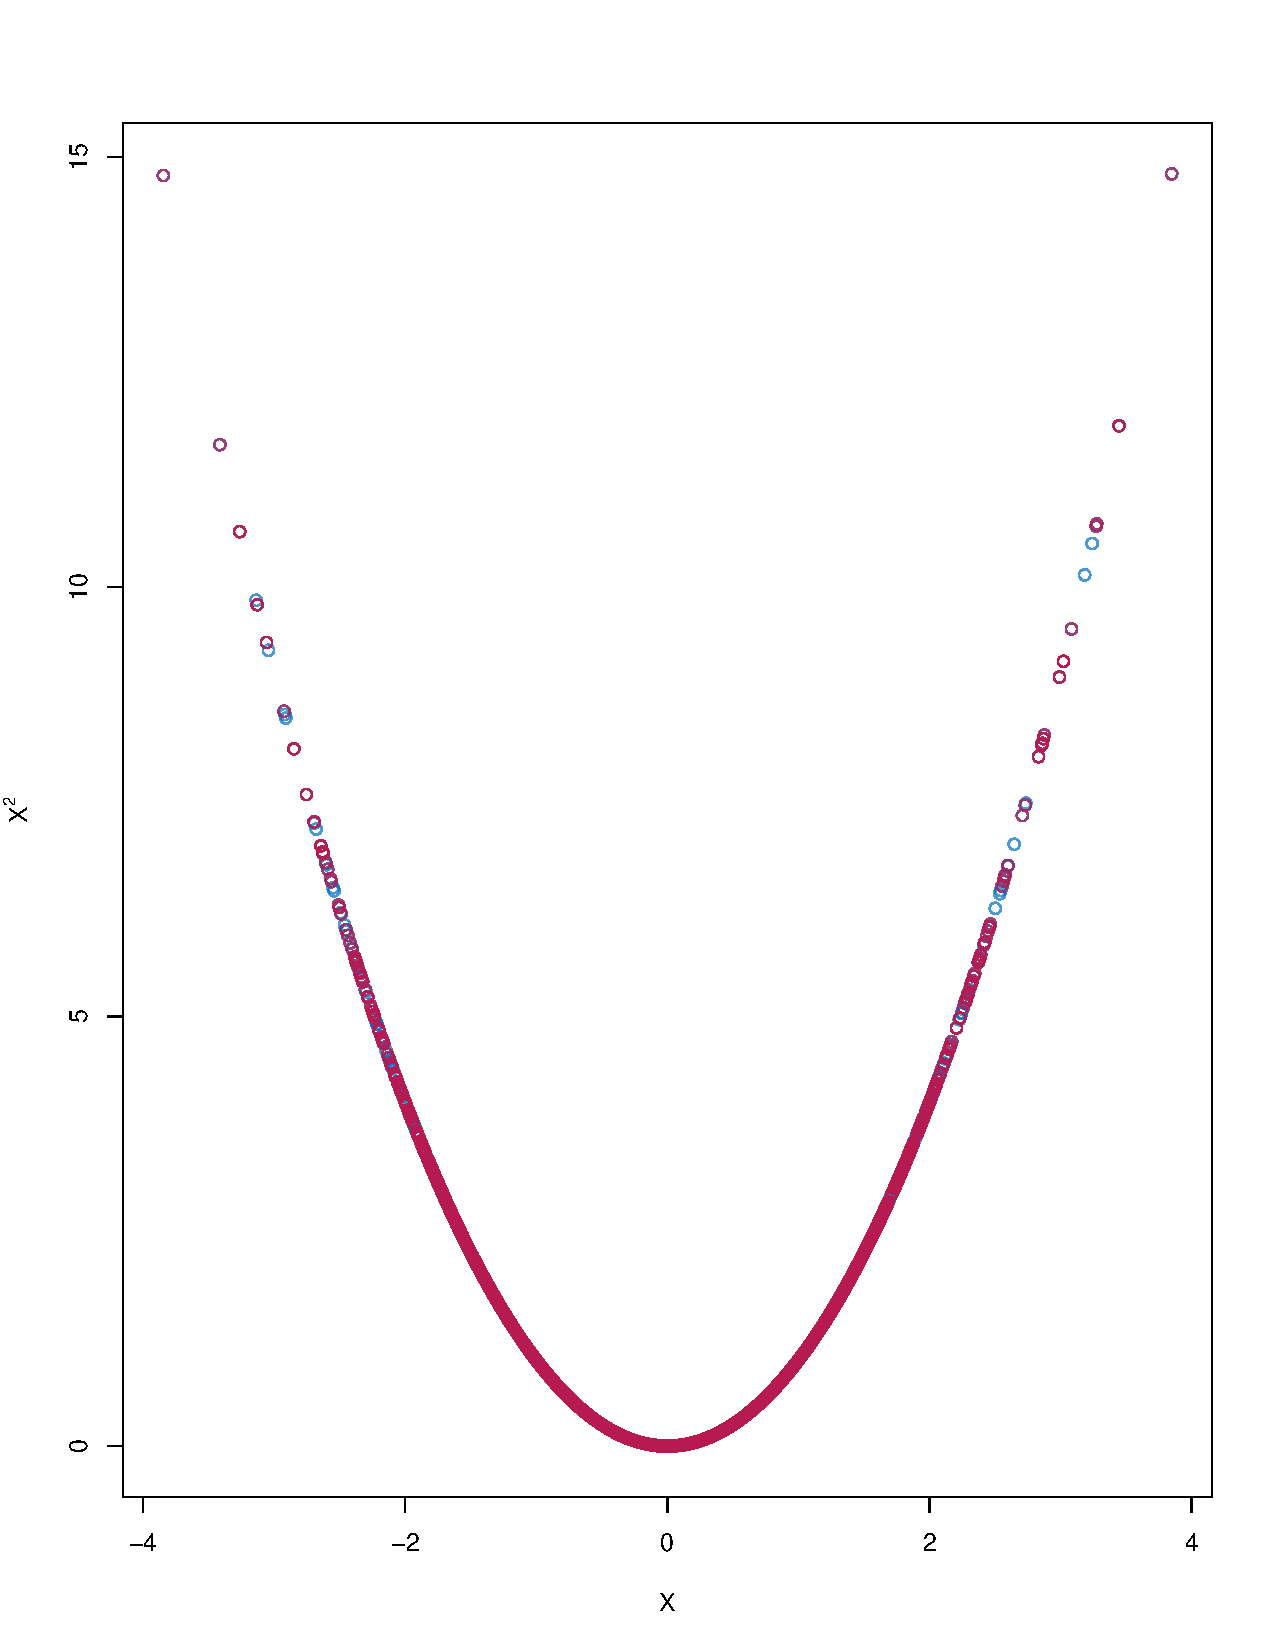
\includegraphics[width=\columnwidth]{plots/plot3.1.pdf}
		\caption{Predictive mean matching based on canonical regression analysis. Observed (blue) and imputed values (red) for $X$ and $X^2$.}
		\label{fig3_1}
	\end{figure}
	
	
	\subsection{Linear regression with interaction term}
	This section considers a linear regression substantive model, which includes two predictors and their interaction effect. 
	
	\subsubsection{Simulation conditions}
	The dependent variable $Y$ was generated according to the analysis model
	\begin{equation}
		\boldsymbol{Y} = \alpha+ \beta_1\boldsymbol{X_1} +  \beta_2\boldsymbol{X_2} + \beta_3\boldsymbol{X_1X_2} + \epsilon
	\end{equation}
	where $\alpha=0$, $\beta_1=1$, $\beta_2=1$, $\beta_3=1$, two predictors $\boldsymbol{X_1}$, $\boldsymbol{X_2}$ and error term $\epsilon$ were assumed as standard normal distributions. Under five types of missingness mechanisms: MCAR, MARleft, MARmid, MARtail, and MARright, the probability of jointly missing $X_1$ and $X_2$ was set to 0.4. There were no units with missing values on either $\boldsymbol{X_1}$ or $\boldsymbol{X_2}$. Missing values were amputed with the \texttt{ampute} function from the package \texttt{MICE} in \texttt{R}. For each simulation scenario, $n=5000$ units were generated and 1000 simulations were repeated.   
	
	\subsubsection{Estimation methods}
	We evaluated and compared the same methods as under section \ref{sec:3.4.1}, except the polynomial combination method. The model-based imputation method ensures a compatible imputation model by accommodating the designed model $\boldsymbol{Y} = \boldsymbol{X_1} + \boldsymbol{X_2} + \boldsymbol{X_1X_2} + \epsilon$. 
	
	
	\subsubsection{Results}
	\begin{table}[ht!]
		\centering
		\resizebox{\textwidth}{!}{
			\begin{tabular}{lcccccrl}
				\hline
				&\multicolumn{5}{c}{Missingness Mechanism} \\
				\cline{2-6}
				&MCAR	&MARleft	&MARmid		&MARtail	& MARright\\
				\hline
				\textit{Transform, then impute}	&&&&&\\
				Intercept ($\alpha$)				&0	&0.05	&-0.05 &0.06	&0.05\\
				Slope of $X_1$ ($\beta_1$)			&1(0.93)		&0.96(0.4)	&1(0.94)	&1.05(0.42)	&1.08(0.05)\\
				Slope of $X_2$ ($\beta_2$)		&1(0.94)		&0.96(0.4)	&1(0.96)	&1.05(0.38)	&1.09(0.02)\\
				Slope of $X_1X_2$($\beta_3$)    &1(0.94)        &0.96(0.53)    &0.95(0.25)    &1.06(0.31)    &1.09(0.02)\\
				Residual SD ($\sigma_\epsilon$) 	&1	&0.97	&1	&1.02	&1.04\\
				$R^2$						&0.75	&0.76	&0.75	&0.74	&0.73\\\\
				\textit{Impute, then transform}	&&&&&\\
				Intercept ($\alpha$)				&0	&-0.04	&-0.01	&0.01	&0.11\\
				Slope of $X_1$ ($\beta_1$)			&0.98(0.88)	&1.05(0.51)	&0.96(0.71)	&0.98(0.9)	&0.95(0.69)\\
				Slope of $X_2$ ($\beta_2$)		&0.98(0.88)	&1.05(0.48)	&0.96(0.73)	&0.98(0.92)	&0.95(0.69)\\
				Slope of $X_1X_2$($\beta_3$)    &0.64(0)  &0.64(0)  &0.7(0)  &0.54(0)  &0.61(0)\\
				Residual SD ($\sigma_\epsilon$) 	&1.25	&1.18	&1.22	&1.28	&1.37\\
				$R^2$						&0.61	&0.65	&0.63	&0.59	&0.53\\\\
				\textit{MPMM}	&&&&&\\
				Intercept ($\alpha$)				&0	&0	&0	&0.01	&0.02\\
				Slope of $X_1$ ($\beta_1$)			&1(0.93)		&1(0.86)		&1(0.92)		&1.02(0.8)	&1.02(0.73)\\	
				Slope of $X_2$ ($\beta_2$)		&1(0.93)		&1(0.84)		&1(0.93)	&1.02(0.8)	&1.02(0.77)\\	
				Slope of $X_1X_2$($\beta_3$)     &1(0.94) &1.01(0.86)   &1(0.93) &1.02(0.71)  &1.03(0.68)\\
				Residual SD ($\sigma_\epsilon$) 	&1		&1.01		&1		&1.03	&1.03\\	
				$R^2$						&0.75	&0.74	&0.75	&0.74	&0.74\\\\
				\textit{SMC-FCS}	&&&&&\\
				Intercept ($\alpha$)				&0	&-0.01	&0	&0.01	&0.03\\
				Slope of $X_1$ ($\beta_1$)			&1(0.95)	&1.01(0.95)	&1(0.95)	&1(0.96)	&0.99(0.95)\\
				Slope of $X_2$ ($\beta_2$)		&0.99(0.94)	&0.99(0.93)	&1(0.97)	&1(0.96)	&0.99(0.96)\\
				Slope of $X_1X_2$($\beta_3$)    &1(0.95)  &1(0.96)  &1(0.95)   &1(0.97)  &1.01(0.93)\\
				Residual SD ($\sigma_\epsilon$) 	&1.02	&1.02	&1	&1.07	&1.06\\
				$R^2$						&0.74	&0.74	&0.75		&0.71	&0.72\\\hline
			\end{tabular}
		}
		\caption{Average parameter estimates for different imputation methods under five different missingness mechanisms over 1000 imputed datasets ($n=5000$) with 40\% missing data. The designed model is $Y = \alpha+ \beta_1X_1 +  \beta_2X_2 + \beta_3X_1X_2 + \epsilon$, where $\alpha=0$, $\beta_1=1$, $\beta_2=1$, $\beta_3=1$ and $\epsilon \sim N (0,1)$. The population coefficient of determination $R^2=.75$. The confidence interval coverages for $\beta_1$, $\beta_2$ and $\beta_3$ are in parentheses. Monte Carlo standard errors for bias are all less than 0.001. Monte Carlo standard errors for confidence interval coverage are less than 1.58\%.}
		\label{tab3_3}
		
	\end{table}
	
	Table \ref{tab3_3} shows the estimates of $\alpha$, $\beta_1$, $\beta_2$, $\beta_3$, $\sigma_\epsilon$, $R^2$ and the coverage of the 95\% confidence intervals for $\beta_1$, $\beta_2$ and $\beta_3$. With MCAR, MARleft, and MARmid, MPMM was unbiased, and the CI coverage for regression weights was at the nominal level. While similar to the linear regression with quadratic term situation, with MARtail and MARright, MPMM yielded unbiased estimates but had relatively reduced confidence interval coverage. The reason is explained in section \ref{sec:3.4.1}. \emph{`Transform, then impute'} method did not preserve the relations even though it resulted in plausible inferences in cases of MCAR and MARmid. The imputations were not plausible. Moreover, with MARleft, MARtial, and MARright, \emph{`transform, then impute'} method gave severely biased estimates and extremely poor CI coverage. \emph{`Impute, then transform'} method generally yielded biased estimates, and the CI for coefficients $\beta_1$, $\beta_2$ and $\beta_3$ had lower than nominal coverage with all five types of missingness. SMC-FCS yielded unbiased estimates of regression weights and had correct CI coverage in all simulation scenarios. The only potential shortcoming of the model-based imputation method was that the estimates of $\sigma_\epsilon$ and $R^2$ showed slight deviations from true values with MARtail and MARright.  
	
	\subsection{Incomplete dataset with inequality restriction $\boldsymbol{X_1} + \boldsymbol{X_2} \geqq C$}
	\label{sec:3.4.3} 
	Multiple predictive mean matching is flexible to model relations among missing variables other than linear regression with polynomial terms or interaction terms. Lastly, we would evaluate the inequality restriction $\boldsymbol{X_1} + \boldsymbol{X_2} \geqq C$, which is relatively difficult for the model-based imputation approach to specify. One application of such inequality restriction would be the analysis of the academic performance of qualified students. For example, the sum score of mid-term and final exams should exceed a fixed value.  
	
	\subsubsection{Simulation conditions} 
	The data was generated from: 
	\begin{eqnarray*}
		\begin{pmatrix}\boldsymbol{X_{1}}\\
			\boldsymbol{X_{3}}
		\end{pmatrix} & \sim & \mathcal{N}\left[\left(\begin{array}{c}
			0\\
			1
		\end{array}\right),\left(\begin{array}{cc}
			4 & 3.2\\
			3.2 & 4
		\end{array}\right)\right],\\
	\end{eqnarray*}
	$\boldsymbol{X_2} = 3 - \boldsymbol{X_1} + \epsilon$, where $\epsilon$ followed a standard uniform distribution. The sum of $\boldsymbol{X_1} + \boldsymbol{X_2} \geqq 3$ was the restriction in the generated data. We simulated missingness such that rows in the block $(\boldsymbol{X_1, X_2,})$ were always either observed or completely missing. We considered 30\% joint missingness of $\boldsymbol{X_1}$ and $\boldsymbol{X_2}$. 2000 subjects were generated and 1000 simulations were performed for two missingness mechanisms : MCAR and MARright. We evaluated the mean of $X_1$ and $X_2$ and the coverage of nominal 95\% CIs. 
	
	\subsubsection{Estimation methods}
	We compared MPMM with PMM to illustrate the limited performance of univariate imputation approaches when there are relations connected to multiple missing variables. We did not apply joint modelling and univariate model-based imputation methods because it is hard to specify the designed inequality restriction.
	
	\subsubsection{Results}
	\begin{table}[ht!]
		\centering
		\resizebox{\textwidth}{!}{
			\begin{tabular}{ccc|cc|cc|cc}
				& \multicolumn{4}{c|}{MPMM}                                & \multicolumn{4}{c}{PMM}                                 \\\hline
				& \multicolumn{2}{c|}{MCAR} & \multicolumn{2}{c|}{MARright} & \multicolumn{2}{c|}{MCAR} & \multicolumn{2}{c}{MARright} \\\hline
				& MEAN      & COVERAGE     & MEAN        & COVERAGE       & MEAN      & COVERAGE     & MEAN        & COVERAGE       \\\hline
				$E(X_1)$ & 0         & 0.95         & 0.01        & 0.94           & 0         & 0.92         & -0.3        & 0              \\\hline
				$E(X_2)$ & 3.5       & 0.95         & 3.51        & 0.95           & 3.5       & 0.92         & 3.8         & 0             
			\end{tabular}
		}
		\caption{Average parameter estimates for MPMM and PMM under MCAR and MARright over 1000 imputed datasets ($n=2000$) with 30\% missing data. The designed model is introduced in section \ref{sec:3.4.3}. The true values of $E(X_1)$ and $E(X_2)$ are $0$ and $3.5$. Monte Carlo standard errors for means are all less than 0.002. Monte Carlo standard errors for confidence interval coverage are less than 0.86\%.}
		\label{tab3_4}
	\end{table}
	
	Table \ref{tab3_4} shows the mean estimates of $\boldsymbol{X_1}$ and $\boldsymbol{X_2}$ and coverage of the corresponding 95\% CIs. The true values for $E(\boldsymbol{X_1})$ and $E(\boldsymbol{X_2})$ are $0$ and $3.5$. MPMM yielded unbiased estimates with MCAR and MARright and had the correct CI coverage. However, PMM was unbiased with close to 95\% when the missingness mechanism is MCAR. It had considerable bias and extremely poor coverage with MARright. The reason is that the relations between $X_1$ and $X_2$ are not modelled \citep{Morris2014}.   
	
	\section{Conclusion}
	\label{sec:3.5}
	Predictive mean matching is an attractive method for missing data imputation. However, because of its univariate nature, PMM may not keep relations between variables with missing units. Our proposed modification of predictive mean matching, MPMM, is a multivariate extension of PMM that imputes a block of variables. We combine canonical regression analysis with predictive mean matching so that the models for donors selection are appropriate when there are restrictions involving more than one variable. MPMM could be valuable because it inherits the advantages of predictive mean matching and preserves relations between partially observed variables. Moreover, since predictive mean matching performs well in a wide range of simulation studies, so can the multivariate predictive mean matching.     
	
	We assess the performance of the multivariate predictive mean matching under three different substantive models with restrictions. In the first two simulation studies, MPMM provides unbiased estimates where the scientific model includes squared terms and interaction terms under both MCAR and MAR missingness mechanisms. However, with MARtail and MARright, MPMM suffers the undercoverage issue because the density of the response indicator is heavy-tailed with our simulation setup. It makes units with large $Y$ almost unobserved and more missing than observed data in the tail region. The missingness mechanism is commonly moderate in practice, unlike MARtial and MARright in simulation studies. Overall, when no sub-regions of the sample space are sparsely observed, the multiple predictive mean matching analysis will provide unbiased estimates and correct CI coverage. 
	
	SMC-FCS yields better estimates and CI coverage of regression weights, but MPMM provides relatively accurate $\sigma_\epsilon$ and $R^2$. The comparison is not entirely fair because SMC-FCS, as used here, requires the correct substantive model for the data. In practice, we often do not know the model, and MPMM becomes attractive. MPMM is an easy-to-use method when there is unit non-response in the survey or the efficiency of estimators is not of great interest. 
	
	The third simulation shows the appealing properties of MPMM. When relations of missing variables are challenging to model, MPMM becomes the most effective approach to imputation. We expect that MPMM could be applied to other relations not yet discussed in section \ref{sec:3.4}.    
	
	We limited our calculations and analyses to normal distributed $\boldsymbol{X}$. However, since Vink (2014) concluded that PMM yields plausible imputations with non-normal distributed predictors, we argue that distributions of predictors will not significantly impact the imputations. We focus on the simple case with one missing data pattern. One possible way to generalize MPMM to more complicated missing data patterns is proposed in the appendix. The general idea is to partition the cases into groups of identical missing data patterns in the block imputed with MPMM. We then perform the imputation in ascending order of the fraction of missing information, i.e., we first impute cases with relatively small missing data problems. Considering to impute partially observed covariates for linear regression with a quadratic term $Y = X + X^2$, we first impute cases with only missing value in $X^2$ by square the observed $X$. Then cases with only missing value in $X$ are imputed with one square root of $Y = X + X^2$. However, the selection of roots should be modelled with logistic regression. Finally, we impute cases with jointly missing $X$ and $X^2$ with MPMM. The comprehensive understanding of MPMM with multiple missing data patterns is an area for further research.         
	
	\section*{Appendix}
	The MPMM algorithm with multiple missing patterns:
	\begin{enumerate}
	\item Sort the rows of $\boldsymbol{Y}$ into $S$ missing data patterns $\boldsymbol{Y_{[s]}}, S=1,\cdots,s$.
	\item Initialize $\boldsymbol{Y_{mis}}$ by a reasonable starting value.
	\item Repeat for $M=1,\cdots,m$.
	\item Repeat for $S=1,\cdots,s$.
	\item Impute missing values by steps 1-8 of MPMM algorithm proposed in section 2.3.
	\item End repeat S.
    \item End repeat M.
\end{enumerate} 
	
	

	


